\section{Introdução}

Dados dois grafos $G_1 = (V, E_1)$ e $G_2 = (V, E_2)$, o problema sanduíche busca encontrar uma determinada propriedade $\Pi$ em um grafo $G' = (V, E')$, onde $E_1 \subseteq E' \subseteq E_2$ onde se quer determinar se o grafo $G'$ pertence a uma família ou classe de grafos, como por exemplo se o grafo ele é cordal ou não. O problema sanduíche vem a ser uma generalização do problema de reconhecimento, onde foi introduzido por Golumbic, Kaplan e Shamir \cite{golumbic:95}. Nesse trabalho será explicado com maiores detalhes a respeito o problema sanduíche e a aplicação do problema para a classes dos grafos split e os grafos cordais.

O problema sanduíche possui aplicações nas áreas de mapeamento físico do DNA, raciocínio temporal, sincronização de processos paralelos, árvores filogenéticas, sistemas esparsos de equações lineares \cite{fernanda:2016}.

O trabalho para esta atividade acadêmica tem como objetivo definir formalmente o problema sanduíche, as classes dos grafos cordais e split e o problema sanduíche para essas duas classes. No primeiro capítulo terá, além da descrição do problema brevemente explicado, algumas definições e conceitos básicos que serão discutidos em capítulos posteriores para melhor compreensão, no capítulo 2 serão definidos formalmente as classes dos grafos cordais e split, no capítulo 3 entraremos em detalhes sobre o problema sanduíche e o capítulo 4 com conclusão do trabalho.

%%e o capítulo 4 será apresentado um algoritmo de força bruta para resolver o problema sanduíche para os grafos cordais, ou seja, se dados dois grafos $G_1$ e $G_2$, se existe um grafo $G'$ "ensanduichado" que pertença a classe dos grafos cordais.%%

\subsection{NP-completude}

Alguns problemas aplicados ao problema sanduíche são classificados como $NP$-completos, para os grafos cordais o problema é considerado $NP$-completo, já para os grafos $split$ existe um algoritmo em tempo polinomial. 

Com relação às classes de $NP$-completude, dizemos que um problema é $P$ caso exista algum algoritmo que resolva um determinado problema $\Pi$ em tempo polinomial, ou seja, que o tempo de execução para resolvê-lo é proporcial ao tamanho de sua entrada, algoritmos que classificamos como eficientes possuem complexidade na ordem polinomial, como $O(n^2), O(n log_n), O(n)$. Um problema é considerado $NP$ quando para um determinado problema $\Pi$ existe uma justificativa SIM para o certificado do problema e um algoritmo complexidade polinomial no passo de reconhecimento, caso não exista, não necessariamente esse problema não pertence a classe $NP$. No problema do caminho hamiltoniano, por exemplo, uma justificativa para seu problema é encontrar um ciclo no grafo tal que ao percorrê-lo, não se repita o caminho por uma aresta, um reconhecimento desse problema seria encontrar a resposta NÃO para o seu certificado, por exemplo, caso não haja um ciclo hamiltoniano qualquer no grafo, então deverão ser verificados todos os ciclos no grafo para fazer essa verificação, para o problema do ciclo hamiltoniano, não é conhecido até então um algoritmo eficiente para resolver o problema em tempo polinomial.

Os problemas da classe $NP$-completos são os mais difíceis da classe $NP$ e provavelmente não façam parte da classe dos problemas $P$, essa classe de problemas são um subconjunto dos problemas $NP$, na figura 1 podemos observar um diagrama com as classes dos problemas. Os problemas $NP$-difíceis são problemas tão difíceis quanto os $NP$-completos, com a diferença que a saída do problema $NP$-difícil torna-o um problema de otimização, maiores detalhes a respeito dessa classe podem ser consultados em \cite{JaymeGrafosNovo}.

Existe um problema em aberto envolvendo as classes de algoritmos $P$ e $NP$ onde se quer encontrar a resposta se $P = NP$. Obviamente, ainda não descobriu se existe algum problema da classe $NP$ que seja intratável, ou seja, que não há um algoritmo que o resolva em tempo polinomial. A resposta para esse problema ainda continua em aberto mas que há evidências que direcionam para $P \neq NP$ devido a classe $NP$ possuir muitos problemas, e mesmo assim não foi encontrado um algoritmo em tempo polinomial que os resolva.

\begin{figure}
    \centering
    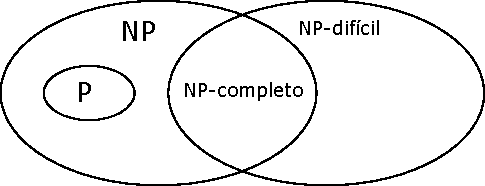
\includegraphics{pictures/diagrama_np.pdf}
    \caption{Diagrama das classes de problemas}
    \label{fig:np_problems}
\end{figure}

\subsection{Definições}

\subsubsection{Esquema de eliminação perfeita}

Um vértice $v$ é considerado simplicial se todos os seus vizinhos $N(v)$ induzirem uma clique maximal do grafo original. Por exemplo, o vértice $a$ do grafo da figura 2 não é simplicial, pois seu vizinho $b$ não induz uma clique maximal.

Um conjunto de vértices ordenados $\phi = v_1, v_2, ..., v_n$ é um esquema de eliminação perfeita se cada vértice $v_i$ removido do conjunto é um vértice simplicial do grafo. Por exemplo, os vértices da figura 1 uma vez ordenados num conjunto $\phi = a, b, c, d$, se para cada vértice removido eles forem simpliciais, então dizemos que existe um esquema de eliminação perfeita.

\subsubsection{Grafos Perfeitos}

Um grafo $G$ é dito perfeito se o número cromático de cada subgrafo induzido for igual ao tamanho da maior clique do subgrafo induzido.

\subsubsection{Grafos Livres}

Um grafo é dito livre de uma determinada propriedade $\Pi$, que podemos usar como exemplo o grafo $K_3$, se não existe em um grafo $G = (V, E)$ um subgrafo com essa propriedade, caso não exista, chamamos esse grafo de $livres$ de triângulos, ou em termos mais práticos, podemos usar a notação $\{K_3\}$-$free$.  

\subsection{Conjunto Independente}

Um conjunto de vértices é dito independente se todos os vértices do conjunto formam componentes desconexas, ou seja, todos os vértices do grafo são isolados, não tendo entre eles nenhuma vizinhança em comum.